\documentclass[11pt]{article}

\usepackage[margin=1in]{geometry}
\usepackage{amsmath,amssymb}
\usepackage{xcolor}
\usepackage{tikz}
\usetikzlibrary{decorations.pathreplacing,arrows.meta,positioning}
\usepackage{booktabs}
\usepackage{tabularx}
\usepackage{enumitem}
\usepackage{graphicx}
\usepackage[colorlinks=true,allcolors=teal!55!black]{hyperref}

\definecolor{inkc}{HTML}{1B2433}
\definecolor{accentc}{HTML}{1F7A7C}
\definecolor{failc}{HTML}{C24A34}
\definecolor{successc}{HTML}{2F7D57}
\definecolor{mutedc}{HTML}{586274}

\newcommand{\cyes}{\textcolor{successc}{$\checkmark$}}
\newcommand{\cno}{\textcolor{failc}{$\times$}}
\newcommand{\arxiv}[1]{\href{https://arxiv.org/abs/#1}{arXiv:#1}}

\newcommand{\callout}[2]{%
  \par\smallskip\noindent
  \fcolorbox{accentc}{accentc!6}{%
    \begin{minipage}{\dimexpr\linewidth-2\fboxsep-2\fboxrule\relax}
      \textbf{\textcolor{accentc}{#1}}\;\; #2
    \end{minipage}}%
  \par\smallskip}

\newcommand{\glance}[4]{%
  \par\smallskip\noindent
  \fcolorbox{mutedc!45}{mutedc!8}{%
    \begin{minipage}{\dimexpr\linewidth-2\fboxsep-2\fboxrule\relax}
      \footnotesize
      \textbf{\textcolor{mutedc}{AT A GLANCE}}\\[3pt]
      \textbf{Q.}~#1\\[2pt]
      \textbf{How.}~#2\\[2pt]
      \textbf{Test.}~#3\\[2pt]
      \textbf{Why it matters.}~#4
    \end{minipage}}%
  \par\smallskip}

\setlength{\parskip}{0.5em}
\setlength{\parindent}{0pt}

\title{\textbf{Catching Silent Failures in LLM Agents}\\[2pt]
       \large Beyond-Score Uncertainty from Diverse Critics --- Research Proposal}
\author{Joseph M. Morante Jr.}
\date{September 2026}

\begin{document}
\maketitle
\vspace{-1.6em}

\glance
  {When an agent selects its next action (or trajectory) using a critic to score candidates, can the critic's \emph{uncertainty} flag the ``silent failures'' --- actions the critic rates highly but that actually derail the task?}
  {Log an agent's candidate actions on verifiable tasks, take the ones it \emph{selects}, and check whether uncertainty adds signal \emph{beyond} the critic score itself --- and whether it depends on the critics being genuinely \emph{diverse}.}
  {$\Delta$AUROC $>0$ among the selected actions, with critic score and cheap features already controlled; and whether it rises with critic diversity.}
  {A calibrated ``this selected action is secretly failing'' signal is exactly the missing trigger for backtracking / selective verification in reliable agents. A clean null is itself a safety-relevant result.}

\callout{Working claim.}{An LLM agent commits to actions by taking the highest-scoring
candidate under a critic (best-of-$n$, tree search, or a process reward model).
Selecting the argmax of an imperfect critic concentrates on the critic's own
mistakes --- the \emph{silent failures} that look good but derail the task. This
project tests whether critic \emph{uncertainty} carries information about those
failures --- conditional on selection, beyond the critic score itself --- and
whether that information is a property of \emph{critic diversity} rather than of
ensembling per se.}

\callout{Research question.}{Among the actions (or trajectories) an LLM agent
selects from a critic's top scores, does critic uncertainty discriminate
task-verified failures from successes \emph{beyond the critic score itself}, and
how does this depend on \emph{critic ensemble diversity}?}

\textit{In plain terms.} An agent's chosen next steps are a mix of real progress
and moves that only \emph{look} like progress to its critic. Among those chosen
moves, does disagreement across a panel of critics reveal the silent failures the
score alone missed --- and only when the panel is genuinely different, not
near-clones?

% ---------------- Figure 1 ----------------
\begin{figure}[t]\centering
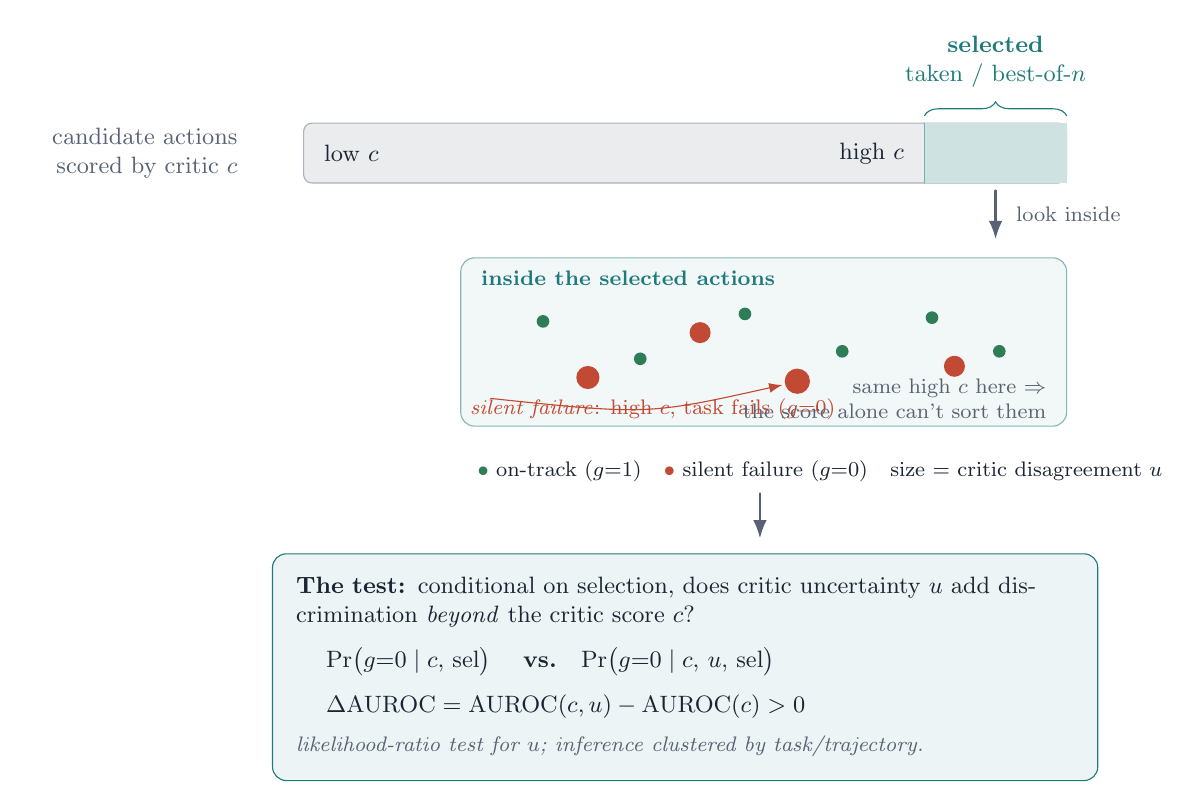
\begin{tikzpicture}[>=Latex, line cap=round, font=\small, inkc, scale=0.95, transform shape]
  \node[mutedc,anchor=east] at (-0.15,5.0) {\begin{tabular}{r}candidate actions\\ scored by critic $c$\end{tabular}};
  \draw[rounded corners=3pt, fill=mutedc!12, draw=mutedc!50] (0.4,4.6) rectangle (10.6,5.4);
  \fill[accentc!22] (8.7,4.6) rectangle (10.6,5.4);
  \draw[accentc!60] (8.7,4.6) -- (8.7,5.4);
  \node[anchor=west] at (0.55,5.0) {low $c$};
  \node[anchor=east] at (8.55,5.0) {high $c$};
  \draw[decorate,decoration={brace,amplitude=5pt},accentc] (8.7,5.5) -- (10.6,5.5);
  \node[accentc,anchor=south,align=center] at (9.65,5.75){\textbf{selected}\\ taken / best-of-$n$};
  \draw[->,mutedc,thick] (9.65,4.5) -- (9.65,3.85);
  \node[mutedc,anchor=west,font=\footnotesize] at (9.8,4.18) {look inside};
  \draw[rounded corners=5pt, draw=accentc!55, fill=accentc!6] (2.5,1.35) rectangle (10.6,3.6);
  \node[accentc,anchor=north west,font=\footnotesize\bfseries] at (2.65,3.55) {inside the selected actions};
  \foreach \p in {(3.6,2.75),(4.9,2.25),(6.3,2.85),(7.6,2.35),(8.8,2.8),(9.7,2.35)}
     \fill[successc] \p circle (2.4pt);
  \fill[failc] (4.2,2.0) circle (4.4pt);
  \fill[failc] (5.7,2.6) circle (4.0pt);
  \fill[failc] (7.0,1.95) circle (4.8pt);
  \fill[failc] (9.1,2.15) circle (4.0pt);
  \draw[failc,->] (2.9,1.72) .. controls (5.0,1.5) .. (6.8,1.9);
  \node[failc,anchor=west,font=\footnotesize,align=left] at (2.5,1.58){\emph{silent failure}: high $c$, task fails ($g{=}0$)};
  \node[mutedc,anchor=east,font=\footnotesize,align=right] at (10.45,1.72){same high $c$ here $\Rightarrow$\\ the score alone can't sort them};
  \node[anchor=west,font=\footnotesize] at (2.6,0.75)
    {\textcolor{successc}{$\bullet$} on-track ($g{=}1$)\quad
     \textcolor{failc}{$\bullet$} silent failure ($g{=}0$)\quad
     size $=$ critic disagreement $u$};
  \draw[->,mutedc,thick] (6.5,0.45) -- (6.5,-0.15);
  \node[draw=accentc, rounded corners=5pt, fill=accentc!8, inner sep=9pt,
        align=left, text width=10.4cm, anchor=north] at (5.5,-0.35)
     {\textbf{The test:} conditional on selection, does critic uncertainty $u$ add
      discrimination \emph{beyond} the critic score $c$?\\[6pt]
      \hspace*{0.4cm}$\Pr\!\big(g{=}0 \mid c,\,\mathrm{sel}\big)$
      \quad\textbf{vs.}\quad
      $\Pr\!\big(g{=}0 \mid c,\, u,\,\mathrm{sel}\big)$\\[6pt]
      \hspace*{0.4cm}$\displaystyle \Delta\mathrm{AUROC}
        = \mathrm{AUROC}(c, u) - \mathrm{AUROC}(c) > 0$\\[4pt]
      {\footnotesize\color{mutedc}\itshape
      likelihood-ratio test for $u$; inference clustered by task/trajectory.}};
\end{tikzpicture}
\caption{An agent's selected actions mix real progress with \emph{silent failures}
that overrated the critic. The estimand asks whether critic uncertainty $u$
discriminates task-verified failures ($g{=}0$) from successes beyond the critic
score $c$, conditional on selection ($\Delta\mathrm{AUROC}>0$).}
\label{fig:agent}
\end{figure}

\section{Background}
\begin{itemize}[leftmargin=1.2em,itemsep=3pt]
  \item \textbf{Agents fail silently, mid-task, and detection is the bottleneck.}
    LLM agents loop, cascade tool errors, drift off-goal, or fabricate success;
    catching these before they compound is the reliability problem, and judging
    every step with a second LLM costs more than the agent itself
    (\textbf{AgentForesight}, \arxiv{2605.08715}; \textbf{Real-Time Detection and
    Repair of Agent Failures}, \arxiv{2608.02464}; survey, \arxiv{2602.05073}).
  \item \textbf{Agents commit by taking the argmax of a critic.} Best-of-$n$, tree
    search, and \emph{process reward models} score candidate steps or trajectories
    and select the top one (\textbf{Let's Verify Step by Step}, \arxiv{2305.20050};
    \textbf{Math-Shepherd}, \arxiv{2312.08935}; \textbf{Generative Verifiers},
    \arxiv{2408.15240}; \textbf{AgentPRM}, \arxiv{2511.08325}). Selecting the
    maximum of an imperfect critic is exactly the operation that surfaces the
    critic's mistakes --- the silent failures that look good to it.
  \item \textbf{Uncertainty tracks reliability --- but only unconditionally, and
    outside agents.} Reward-model ensemble uncertainty filters low-quality outputs
    (\textbf{URM/URME}, \arxiv{2410.00847}; ensembles, \arxiv{2310.02743};
    diversity, \arxiv{2312.09244}) and over-optimization worsens with pressure
    (\arxiv{2210.10760}) --- but shown \emph{marginally}, on single-answer
    non-agentic tasks, never conditioned on the critic score in the selected set.
  \item \textbf{Self-correction needs a trigger.} Reflexion-style verbal
    self-correction and state rollback can recover from a bad step \emph{if they
    know when to fire} (\textbf{Reflexion}, \arxiv{2303.11366}). A calibrated
    ``this selected action is secretly failing'' signal is precisely that missing
    trigger.
\end{itemize}

\section{Gap / Novelty}
No published work asks the agentic, \emph{selection-conditional, beyond-score}
question: among the actions an agent \emph{selects}, does critic \emph{uncertainty}
catch silent failures beyond the critic score, with critic \emph{diversity
manipulated and mediated}, and gold from \emph{task success}. Prior agent work
either scores steps (PRMs, generative verifiers), reflects/repairs after a known
failure (Reflexion), or detects failures without asking whether uncertainty adds
over the score in the selected set. The contribution is three tests:
(i)~\emph{detection} --- does critic uncertainty carry silent-failure information
beyond the score, conditional on selection; (ii)~\emph{mechanism} --- does critic
diversity govern it via error decorrelation (``more critics'' vs ``different
critics''); (iii)~\emph{practice} --- how much survives cheap uncertainty
estimators, and what it buys as a backtrack / selective-verification trigger.

\section{Hypotheses}
\begin{description}[leftmargin=0em,itemsep=3pt]
  \item[H1 (beyond-score detection at selection).] Among selected actions, critic
    uncertainty adds discrimination beyond the critic score ($\Delta\text{AUROC}>0$,
    LR test); the increment shrinks as selection pressure grows (larger $n$, greedier
    argmax), because selection concentrates on the critics' shared blind spots.
  \item[H2 (diversity, mediated).] The increment rises as critics get more diverse
    (seed $\to$ data $\to$ base model $\to$ public-critic zoo), mediated by error
    decorrelation: a diversity step that fails to decorrelate critic errors fails to
    raise $\Delta$AUROC.
  \item[H3 (pressure $\times$ diversity).] The decay of $\Delta$AUROC under stronger
    selection is flatter for base-diverse critic panels: diversity buys robustness to
    optimization pressure, not just level.
  \item[H4 (cheap uncertainty).] Single-critic uncertainty (dropout, quantile-width,
    generative-verifier self-consistency) is tested against true critic ensembles on
    the same estimand; parity and gap are both headlines.
  \item[H5 (failure taxonomy).] Detection is heterogeneous by failure class
    (tool/execution error, goal drift, hallucinated success, doom-loop repetition,
    verifier gaming), and per-class critic error correlation explains it: classes
    where diverse critics fail independently are the classes uncertainty catches.
\end{description}
\textbf{Falsification is informative.} $\Delta$AUROC null even with diverse critics
$\to$ ``beyond-score critic uncertainty carries no silent-failure information ---
agent safeguards built on it inherit the critic's blind spots.'' H2 flat $\to$
diversity doesn't rescue detection. H1 holds, H3 fails $\to$ uncertainty helps only
under mild selection; report the operating envelope.

\section{Formal Problem Definition and Estimand}
\textbf{Setup.} A frozen agent $\pi$ runs on tasks $x\in\mathcal{X}$ from verifiable
benchmarks. At each decision point it produces candidate actions (or whole
trajectories) scored by a critic $c$ (a process reward model, generative verifier,
or LLM judge). Two selection constructions, both reported: (a)~\emph{fixed-percent}
--- the top $k\%$ of candidates by $c$; (b)~\emph{taken / best-of-$n$} --- the
action the agent actually commits to over draws of size $n$, the deployment-relevant
set, with pressure $\mathrm{KL}\approx \log n - (n-1)/n$.

\textbf{Gold.} $g\in\{0,1\}$: at the \emph{trajectory} level, task success (tests
pass / environment reward) --- clean and free on verifiable benchmarks. At the
\emph{step} level, ``the step lies on a still-succeeding path,'' estimated by
Monte-Carlo rollouts from that state (the Math-Shepherd construction), reported with
a rollout-noise sensitivity analysis.

\textbf{Estimand (primary).} The incremental discrimination of uncertainty $u$ over
critic score $c$, conditional on selection:
\[
\underbrace{\Pr\!\big(g{=}0 \mid c,\ \mathrm{sel}\big)}_{\text{base}}
\quad\text{vs.}\quad
\underbrace{\Pr\!\big(g{=}0 \mid c,\ u,\ \mathrm{sel}\big)}_{\text{full}},
\qquad
\Delta\mathrm{AUROC} = \mathrm{AUROC}(c,u) - \mathrm{AUROC}(c).
\]
Report $\Delta$AUROC, partial AUC (low-alarm-rate regime), and the likelihood-ratio
test for $u$, with inference clustered by task/trajectory. The selection-induced
correlation between $c$ and $u$ is reported as a range-restriction diagnostic.

\textbf{Uncertainty $u$.} Primary: disagreement across a critic ensemble
$\{c_1\dots c_m\}$ (std / range / rank disagreement). Cheap: dropout, quantile-width,
generative-verifier self-consistency. Trivial covariates always in the model: critic
score, action length, step index, and the agent's own token entropy.

\textbf{Critic diversity (manipulated).} seed $\to$ data $\to$ base model $\to$
public-critic zoo, with diversity \emph{measured} (pairwise error correlation on
gold, on the full candidate set and the selected set; prediction disagreement; CKA).

\section{Design, Statistical Plan, and Experiments}
\textbf{Fractional design.} An anchor --- base-diverse critics, $m{=}4$,
ensemble-std, best-of-$n{=}16$, $k{=}5\%$, SWE-bench-Verified gold, one open agent
scaffold --- plus one-factor-at-a-time sweeps. \textbf{Pre-registration:} primary
endpoint is $\Delta$AUROC at the anchor, diverse vs seed critics, clustered-bootstrap
95\% CI; other contrasts under Benjamini--Hochberg FDR. \textbf{Confounds:} action
length, step index, agent entropy always in the conditional model; range-restriction
diagnostic; rollout-noise sensitivity for step-level gold.

\renewcommand{\arraystretch}{1.2}
\begin{table}[h]\footnotesize\centering
\begin{tabularx}{\textwidth}{@{}l l X X l@{}}
\toprule
\textbf{ID} & \textbf{Question} & \textbf{Design} & \textbf{Metrics} & \textbf{Tier}\\
\midrule
E1 & Beyond-score detection (H1) & anchor $\pm$ selection sweep ($n$, $k$, taken set) & $\Delta$AUROC, partial AUC, LR vs $n$, $k$ & Core\\
E2 & Critic diversity $+$ mediation (H2) & diversity sweep $\times\, m$ at anchor & $\Delta$AUROC by diversity; error-corr. mediation & Core\\
E3 & Pressure $\times$ diversity (H3) & seed vs base-diverse $\times$ $n$ grid & slope of $\Delta$AUROC in $\log n$ & Core\\
E4 & Cheap uncertainty (H4) & estimator sweep at anchor & incremental $\Delta$AUROC per estimator & Ablation\\
E5 & Failure taxonomy (H5) & labeled failures across classes & per-class $\Delta$AUROC; per-class error corr. & Mechanism\\
E6 & Generality & anchor across SWE-bench / WebArena / ALFWorld & cross-benchmark agreement & Robustness\\
E7 & Backtrack / selective verify (offline) & best cells; logged-trajectory simulation & failures caught at $b\%$ budget; risk--coverage & Impact\\
E8 & Trajectory- vs step-level gold & task-success vs rollout labels & agreement; step-level $\Delta$AUROC & Scope\\
\bottomrule
\end{tabularx}
\end{table}

\section{Doubts / Risks}
\begin{itemize}[leftmargin=1.2em,itemsep=2pt]
  \item \textbf{Step-level gold is the hard part.} ``Was this step a mistake'' is not
    directly verifiable; the MC-rollout label (Math-Shepherd style) is an
    approximation --- so trajectory-level gold (task success) is the clean primary,
    step-level the flagged extension, with rollout-noise sensitivity.
  \item \textbf{The null is publishable and safety-relevant.} If uncertainty adds
    nothing beyond the critic score even with diverse critics, agent safeguards
    built on it inherit the critic's blind spots --- a result worth stating.
  \item \textbf{Range restriction is the crux, not a nuisance.} Selection ties $c$
    and $u$ together in the selected set; the estimand controls for $c$ by
    construction and the induced correlation is reported directly.
  \item \textbf{Critic panels are heterogeneous.} Different critics use different
    formats/scales; scores are rank-normalized before measuring disagreement, and
    per-critic quality (RewardBench-style) is reported.
  \item \textbf{Offline scope for E7.} Adaptive backtrack-then-retry creates
    selection feedback a fixed log cannot simulate; policy simulation is offline in
    v1, with the caveat in limitations.
\end{itemize}

\section{Benchmarks}
\begin{itemize}[leftmargin=1.2em,itemsep=3pt]
  \item \textbf{SWE-bench / SWE-bench Verified} (\arxiv{2310.06770}) --- primary:
    coding agents, gold $=$ unit tests pass; clean, objective trajectory-level labels.
  \item \textbf{WebArena} (\arxiv{2307.13854}) --- long-horizon web tasks with
    checkable success; the goal-drift / doom-loop regime.
  \item \textbf{ALFWorld} (\arxiv{2010.03768}) --- embodied/text household tasks with
    programmatic success; a third, distinct domain for generality (E6).
  \item \textbf{Critics}: process reward models (\arxiv{2305.20050};
    \arxiv{2312.08935}), generative verifiers (\arxiv{2408.15240}), agent PRMs
    (\arxiv{2511.08325}), and public reward models from Hugging Face for the
    maximal-diversity zoo. Per-critic quality anchored to RewardBench (\arxiv{2403.13787}).
\end{itemize}
Metrics: $\Delta$AUROC and partial AUC (primary), LR test, unconditional AUROC
(secondary), per-class $\Delta$AUROC, error-correlation mediation, and --- for E7 ---
silent failures caught at a $b\%$ backtrack/verification budget with risk--coverage.

\section{Positioning}
\begin{table}[h]\footnotesize\centering
\resizebox{\textwidth}{!}{%
\begin{tabular}{@{}l c c l c c c@{}}
\toprule
\textbf{Work} & \textbf{Selection-} & \textbf{Task-} & \textbf{Uncertainty} &
\textbf{Beyond-} & \textbf{Critic diversity} & \textbf{Failure}\\
 & \textbf{focused} & \textbf{verified} & \textbf{as detector} &
\textbf{score} & \textbf{manipulated} & \textbf{taxonomy}\\
\midrule
PRMs (\arxiv{2305.20050}; \arxiv{2312.08935}) & partial & \cyes & \cno\,(scoring) & \cno & \cno & \cno\\
Generative Verifiers (\arxiv{2408.15240}) & partial & \cyes & \cno\,(scoring) & \cno & \cno & \cno\\
AgentPRM (\arxiv{2511.08325}) & \cyes & \cyes & \cno\,(scoring) & \cno & \cno & \cno\\
Reflexion (\arxiv{2303.11366}) & \cno & \cyes & \cno\,(repair) & \cno & \cno & \cno\\
Agent failure detection (\arxiv{2605.08715}; \arxiv{2608.02464}) & \cyes & \cyes & \cyes & \cno & \cno & partial\\
URM/URME (\arxiv{2410.00847}) & \cno & \cno\,(BoN qual.) & \cyes\,uncond. & \cno & \cno\,(seed) & \cno\\
\midrule
\textbf{This work} & \cyes & \cyes & \cyes & \cyes & \cyes\,4-lvl, mediated & \cyes\\
\bottomrule
\end{tabular}}
\end{table}
\textbf{Open cell:} selection-conditional, beyond-score silent-failure detection in
agents, task-verified, with critic diversity manipulated and mediated.

\section{Value / Feasibility}
Runs on frozen open agents and off-the-shelf / lightly-trained critics: log
trajectories once on open benchmarks, score with a critic panel, label gold from task
success, then the whole study is offline scoring plus regression --- \emph{no RL},
single node. The public-critic zoo is essentially free (download $+$ inference). The
payoff is a calibrated silent-failure trigger for backtracking / selective
verification --- directly the reliable-agent loop --- and a mechanistic account
(diversity $\to$ decorrelation) of when it works. \textbf{Staged:} Stage 0
(vacuousness/power: do silent failures exist in the selected set? is the failure rate
workable? do trivial features saturate?) $\to$ Stage 1 (pre-registered anchor $+$
diversity ladder; a signal promotes, a flat result is a negative-result paper) $\to$
Stage 2 (full matrix E1--E8, three benchmarks, taxonomy, step-level gold).

\section*{References}
\small
\begin{itemize}[leftmargin=1.2em,itemsep=1pt]
  \item Lightman et al. Let's verify step by step (2023). \arxiv{2305.20050}.
  \item Wang et al. Math-Shepherd: verify and reinforce LLMs step-by-step (2023). \arxiv{2312.08935}.
  \item Zhang et al. Generative verifiers: reward modeling as next-token prediction (2024). \arxiv{2408.15240}.
  \item AgentPRM: process reward models for LLM agents via step-wise promise and progress (2025). \arxiv{2511.08325}.
  \item Shinn et al. Reflexion: language agents with verbal reinforcement learning (2023). \arxiv{2303.11366}.
  \item Jimenez et al. SWE-bench: can language models resolve real-world GitHub issues? (2023). \arxiv{2310.06770}.
  \item Zhou et al. WebArena: a realistic web environment for autonomous agents (2023). \arxiv{2307.13854}.
  \item Shridhar et al. ALFWorld: aligning text and embodied environments (2020). \arxiv{2010.03768}.
  \item AgentForesight: online auditing for early failure prediction in multi-agent systems (2026). \arxiv{2605.08715}.
  \item Real-time detection and repair of LLM agent failures (2026). \arxiv{2608.02464}.
  \item Uncertainty quantification in LLM agents: foundations and challenges (survey, 2026). \arxiv{2602.05073}.
  \item URM / URME: uncertainty-based reward modeling and filtering (ICLR 2025). \arxiv{2410.00847}.
  \item Coste et al. Reward model ensembles help mitigate overoptimization (2023). \arxiv{2310.02743}.
  \item Eisenstein et al. Helping or herding? reward-model ensembles (2023). \arxiv{2312.09244}.
  \item Gao, Schulman \& Hilton. Scaling laws for reward model overoptimization (2022). \arxiv{2210.10760}.
  \item Lambert et al. RewardBench: evaluating reward models (2024). \arxiv{2403.13787}.
\end{itemize}

\end{document}
